\documentclass[a4paper]{article}   %文类(论文)
%目录层级
\setcounter{secnumdepth}{4}
\setcounter{tocdepth}{4}
% 宏包
\usepackage{ctex}              	    %支持中文
\usepackage{amsmath}           	    %数学公式
\usepackage{amssymb}
\usepackage{graphicx}          	    %插图
\usepackage{listings}          	    %插入代码
\usepackage{color, xcolor}     	    %颜色
\usepackage{longtable, booktabs}	%三线表
\usepackage{pdfpages}			    %导入pdf
\usepackage{titlesec}			    %设置标题、子标题
\usepackage{subfigure}			    %子图
\usepackage{tcolorbox}			    %彩色盒子
\usepackage{multirow}			    %不规则表格
\usepackage{ulem}				    %下划线
\usepackage{tikz}
\usepackage[hidelinks]{hyperref}	% 超链接

%页边距调整
\usepackage[left=2.54cm, bottom=3.18cm, right=2.54cm, top=3.18cm]{geometry}

\hypersetup
{
	colorlinks = true,
	linkcolor = blue,
	urlcolor = orange,
	citecolor = gray,
}

%设置标题、子标题字体(四号、小四、黑体)
\titleformat*{\section}{\centering \Large \heiti}
%\titleformat{\subsection}{\large \heiti}
%\titleformat{\subsubsection}{\large \heiti}

%设置代码
\lstset{
	basicstyle          =   \sffamily,          % 基本代码风格
	keywordstyle        =   \bfseries,          % 关键字风格
	commentstyle        =   \rmfamily\itshape,  % 注释的风格,斜体
	stringstyle         =   \ttfamily,  % 字符串风格
	flexiblecolumns,                % 别问为什么,加上这个
	numbers             =   left,   % 行号的位置在左边
	showspaces          =   false,  % 是否显示空格,显示了有点乱,所以不现实了
	numberstyle         =   \zihao{-5}\ttfamily,    % 行号的样式,小五号,tt等宽字体
	showstringspaces    =   false,
	captionpos          =   t,      % 这段代码的名字所呈现的位置,t指的是top上面
	frame               =   single,   % 显示边框
%	emph        		=   {self},
%	emphstyle       	=   \bfseries\color{Rhodamine},
}
\lstdefinestyle{Python}{
	language        =   Python, % 语言选Python
	basicstyle      =   \zihao{-5}\ttfamily,
	numberstyle     =   \zihao{-5}\ttfamily,
	keywordstyle    =   \color{blue},
	keywordstyle    =   [2] \color{teal},
	stringstyle     =   \color{magenta},
	commentstyle    =   \itshape\color{red}\ttfamily,
	emph        	=   {self},
	emphstyle       =   \color{purple},
	breaklines      =   true,   % 自动换行,建议不要写太长的行
	columns         =   fixed,  % 如果不加这一句,字间距就不固定,很丑,必须加
	basewidth       =   0.5em,
}

\begin{document}
	%导入模板pdf
	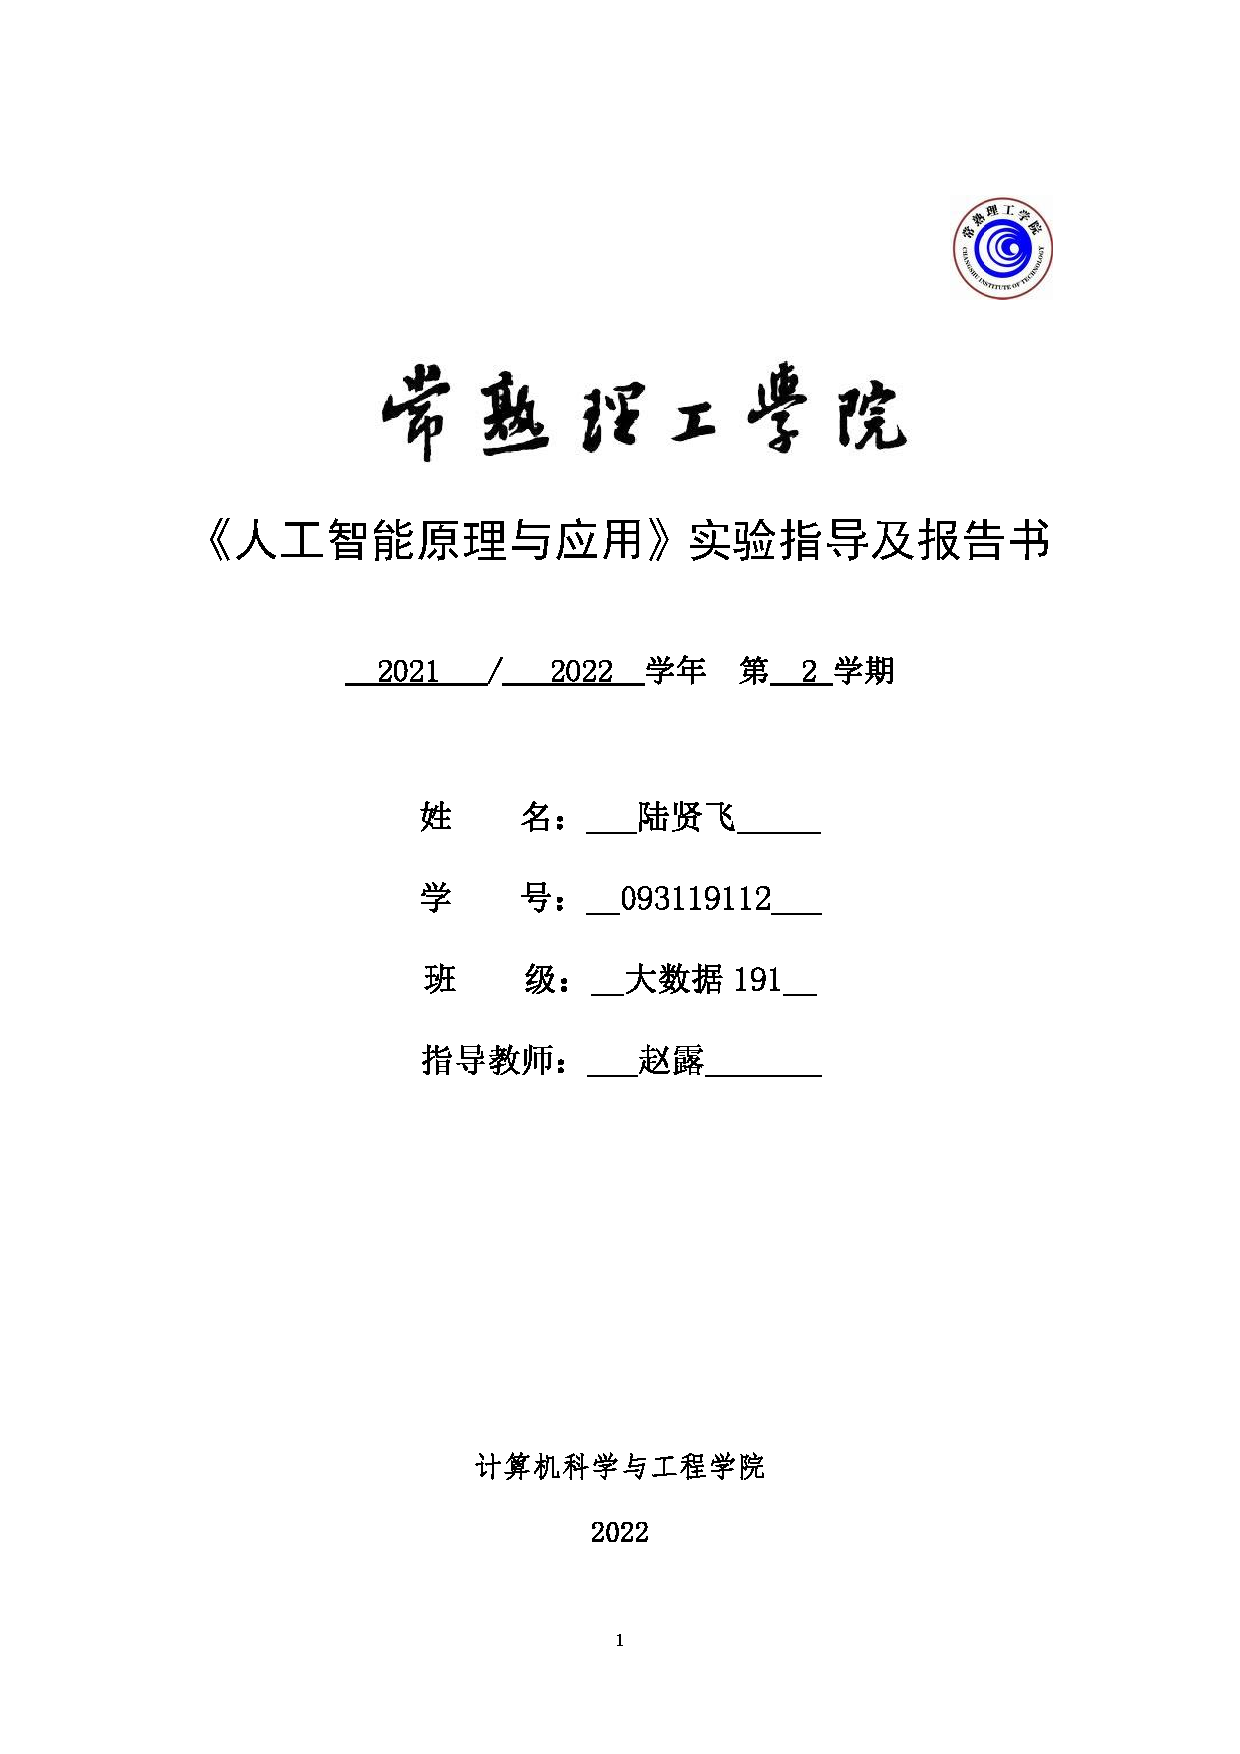
\includepdf[pages={1}]{./resource/header.pdf}
	%小四号字体
	\zihao{-4}
 	\newpage
 	\section*{实验二\quad 动物识别系统}
 	\subsection*{一 \quad 实验目的}
 	熟悉和掌握产生式系统的运行机制,掌握基于规则推理的基本方法。
 	\subsection*{二 \quad 实验原理}
 	产生式系统用来描述若干个不同的以一个基本概念为基础的系统,这个基本概念就是产生式规则或产生式条件和操作对。在产生式系统中,论域的知识分为两部分:用事实表示静态知识;用产生式规则表示推理过程和行为。\par
 	\begin{figure}[!htbp]
 		\centering
 		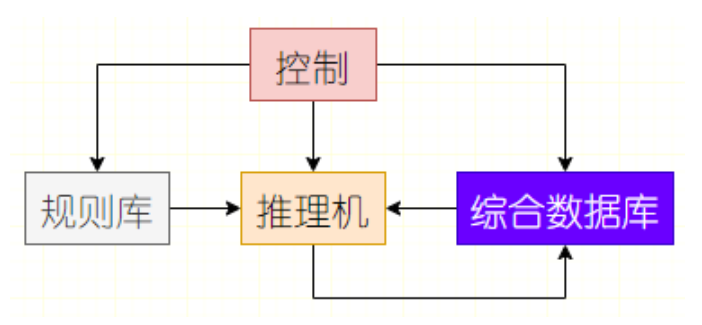
\includegraphics[scale=0.8]{./resource/f1.png}
 	\end{figure}
 	规则库:用于描述相应领域内知识的产生式集合。\par 
 	综合数据库:用于存放问题求解过程中各种当前信息的数据结构。\par 
 	控制系统:由程序组成,负责整个产生式系统的运行,实现对问题的求解。\par 
 	\subsection*{三 \quad 实验内容}
 	\subsubsection*{1. \quad 简述产生式系统的正向推理的过程}
 	正向推理是一种从已知事实出发、正向使用推理规则的推理方式。 \par 
 	\begin{tcolorbox}
 		[colframe=blue!25,
   		colback=blue!10,
   		coltitle=blue!20!black,  
   		fonttitle=\bfseries,
   		adjusted title=Note:
   		]
   		\begin{itemize}
   			\item 用户需要事先提供一组初始证据。 并将其放入综合数据库
   			\item 推理开始后,推理机根据综合数据库中的已有事实,到知识库中寻找当前可用的知识,形成一个当前可用的知识集
   			\item 然后按照冲突消解策略,从该知识集中选择一条知识
   			\item 使用选定的知识进行推理,并将新推出的事实加入综合数据库中,作为后面继续推理时可用的已知事实
   			\item 如此重复直到求出所需要的解或者知识库中再无可用知识为止
   		\end{itemize}
 	\end{tcolorbox}
 	\subsubsection*{2. \quad 编程实现动物识别系统}
 	\noindent
 	\textbf{2.1 根据以下15条规则,建立规则库} \par 
 	\begin{figure}[!htbp]
 		\centering
	 	\subfigure{
	 		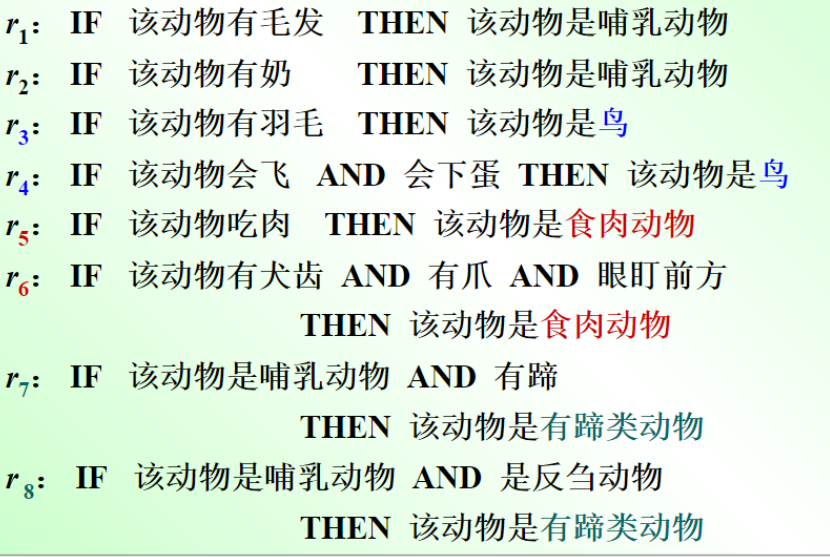
\includegraphics[scale=0.5]{./resource/f2.png}
	 	}
	 	\subfigure{
	 		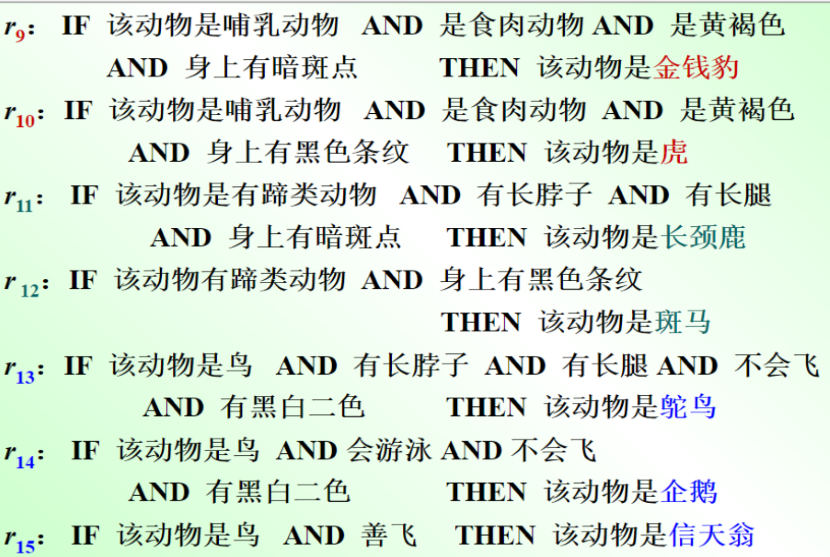
\includegraphics[scale=0.5]{./resource/f3.png}
	 	}
 	\end{figure}
 	\noindent
 	\textbf{2.2 实现推理,打印推理过程} \par
 	\noindent
 	\textbf{2.2.1} 算法主要思路 \par 
 	设映射$ f: R \rightarrow C $,其中$ R $是由上述$ 15 $条规则的条件构成集合,$ C $是由上述$ 15 $条规则的结论构成的集合。容易知道$ f $是一个满射,则对任意$ y \in C $,都存在$ x \in R $,使得$ f(x) = y $,例如
 	\begin{equation*}
 		f(\{\text{会飞}, \text{下蛋}\}) = \text{鸟}
 	\end{equation*} \par
 	于是可以把输入的事实看成一个集合$ I $,如果$ I \in R $,那么存在某个$ y \in C $,使得$ f(I) = y $,如果$ I \notin R $,如果能通过\textbf{添加元素规则}向$ I $中添加有限个元素后,得到成$ I' $,使得$ I'=I_1 \cup \cdots \cup I_n $,其中$ I_i \in R \quad (\forall i = 1, 2, \cdots, n) $,则在这种\textbf{添加元素规则}下,集合$ I $可以推出的结论为$ f(I_n) $,否则集合$ I $不能推出任何结论。下面定义\textbf{添加元素规则:} \par 
 	\textbf{定义2.2.1} 如果有$ I \notin R $,$ I_1, I_2, \cdots I_r \in R $,且$ I_1 \subset I $,那么就令
 	\begin{equation*}
 		I_{r+1} = \left(I - \sum\limits_{i=1}^{r}I_i\right) \bigcup\limits_{i=1}^{r} \{f(I_i)\}
 	\end{equation*}
 	若$ I_{r+1} \in R $,则记。
 	\begin{equation*}
 		I' = \bigcup\limits_{i=1}^{r+1} I_i
 	\end{equation*}
 	\par 
 	举例说明上述思想的正确性,令
 	\begin{equation*}
 		I = \{\text{毛发}, \text{吃肉}, \text{黄褐色}, \text{黑色条纹}\}
 	\end{equation*}
 	显然$ I \notin R $,故用添加元素规则添加元素,首先有$ I_1 = \{\text{毛发}\} $,$ I_2 = \{\text{吃肉}\} $,且$ I_1, I_2 \subset I $,$ I_1, I_2 \in R $,则有
 	\begin{equation*}
 		I_3 = I - I_1 - I_2 \cup \{f(I_1), f(I_2)\} = \{\text{哺乳动物}, \text{食肉动物}, \text{黄褐色}, \text{黑色条纹}\} \in R
 	\end{equation*}
 	此时$ I' = I_1 \cup I_2 \cup I_3 $,于是$ I $ 可以推出的结论为$ f(I_3) = \text{虎} $ \par 
 	用$ Python $中的集合数据结构容易实现,代码如下({\color{blue}其余代码均在附录}):\par
 	\begin{lstlisting}[style=Python]
 		    def deduce(self, keywords):
 		        """
 		        description: 进行推理
 		        param: keywords 关键词集合
 		        Returns: None
 		        """
 		        
 		        # 用于存放推理各步结论
 		        self.conclusion = list()
 		        while len(keywords) != 0:
 		            flag = 0
 		            for rule in self.rulebase:
 		                flag += 1
 		                # 判断集合R中是否有元素是输入事实的子集
 		                if rule.condition.issubset(keywords):
 		                    # 减去该子集
 		                    keywords = keywords - rule.condition
 		                    # 添加子集的结论
 		                    self.conclusion.append(rule)
 		                    if len(keywords) != 0:
 		                        keywords.add(rule.conclusion)
 		                        flag = 0
 		                        continue
 		                    else:
 		                        break
 		            if flag == len(self.rulebase) and len(keywords) != 0:
 		                self.conclusion = list()
 		                break
 	\end{lstlisting}
 	读入规则集
 	\begin{lstlisting}[style=Python]
 		    def initialize_rulebase(self):
 		        """
 		        description: 从本地txt文件中读入规则
 		        param: None
 		        Returns: None
 		        """
 		
 		        with open(file=self.path, mode='r', encoding='utf_8') as file:
 		            rules = file.read().split("\n")
 		            for rule in rules:
 		                if len(rule) != 0:
 		                    self.rulebase.append(Rule(rule.split(" ")))
 	\end{lstlisting}
 	\newpage
 	\noindent
 	\textbf{2.2.2} 推理系统演示 \par 
 	\begin{figure}[!htbp]
 		\centering
 		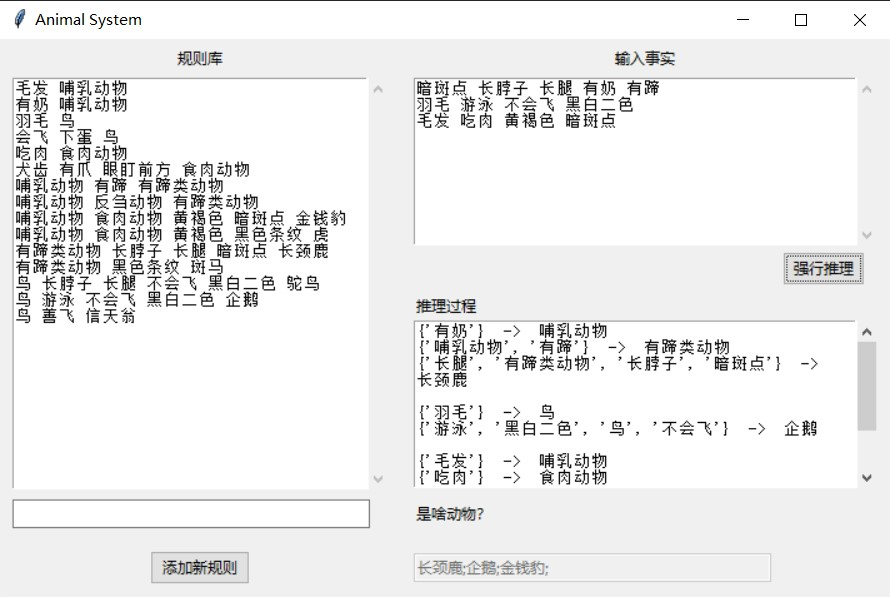
\includegraphics[scale=0.75]{./resource/show1.jpg}
 		\caption{演示推理}
 	\end{figure}
 	\begin{figure}[!htbp]
 		\centering
 		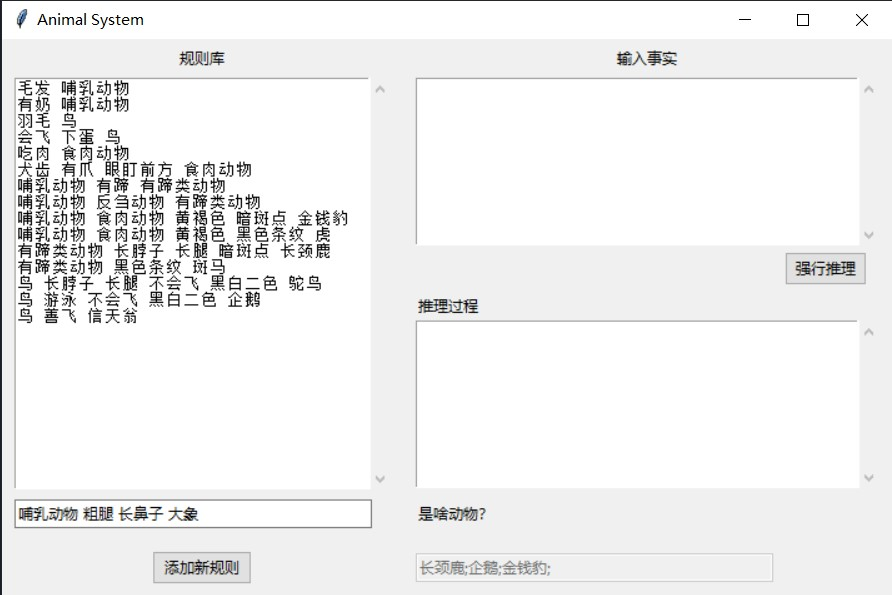
\includegraphics[scale=0.75]{./resource/show2.jpg}
 		\caption{添加规则}
 	\end{figure}
 	\begin{figure}[!htbp]
 		\centering
 		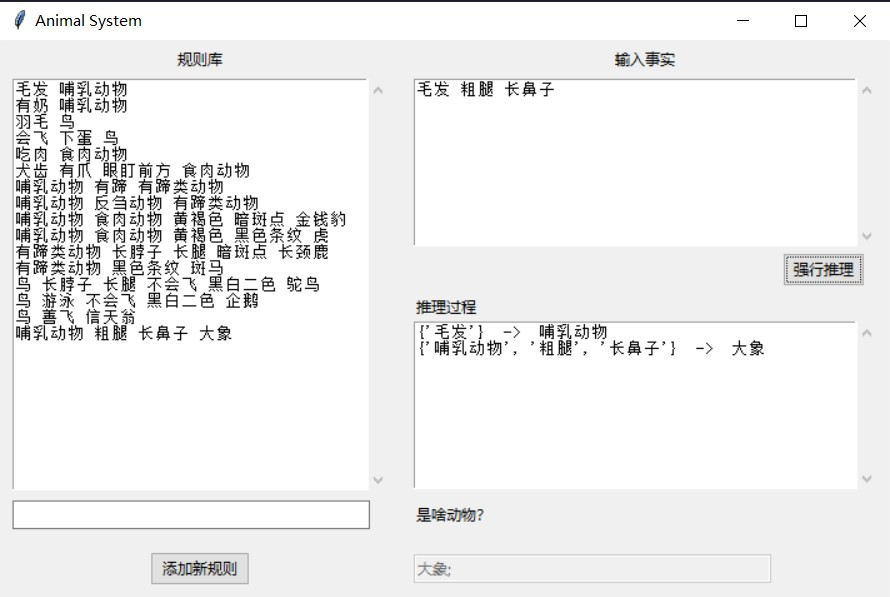
\includegraphics[scale=0.75]{./resource/show3.jpg}
 		\caption{对添加的规则进行测试}
 	\end{figure}
 	\subsection*{提交至$ github $链接}
 	\noindent
 	\href{https://github.com/cgxf2021/AnimalSystem}{https://github.com/cgxf2021/AnimalSystem} 
 	\subsection*{附录}
 	\lstinputlisting[
 		style=Python,
 		caption={\bf animal\_system.py}
 	]{../code/animal_system.py}
 	\lstinputlisting[
 		style       =   Python,
		caption     =   {\bf form.py},
 	]{../code/form.py}
 	
\end{document}